\documentclass[parskip=full]{scrartcl}

\usepackage[utf8]{inputenc}			% Umlaute, Sonderzeichen
\usepackage[ngerman]{babel}			% deutsche Sprache
\usepackage{enumitem}				% Listen
\usepackage{graphicx}				% Grafiken
\usepackage{hyperref}				% Hyperlinks
\usepackage[nonumberlist]{glossaries}		% Glossar
\usepackage{amsmath}
\usepackage{pdfpages}				% PDF einbinden


\makenoidxglossaries



\subject{Benutzerhandbuch}
\title{Handbuch zur Benutzung der Anwendung "FreeJDAQ"}
\subtitle{Version 1.0.0}
\author{David Gawron \and Stefan Geretschläger \and Leon Huck \and Jan Küblbeck \and Linus Ruhnke}
\date{\today}


\begin{document}

\maketitle

\clearpage
\tableofcontents 					% generate pdf twice to update

\section{Einleitung}

\section{Beschreibung der graphischen Benutzeroberfläche}

\begin{figure}[htbp]
    \begin{center}
        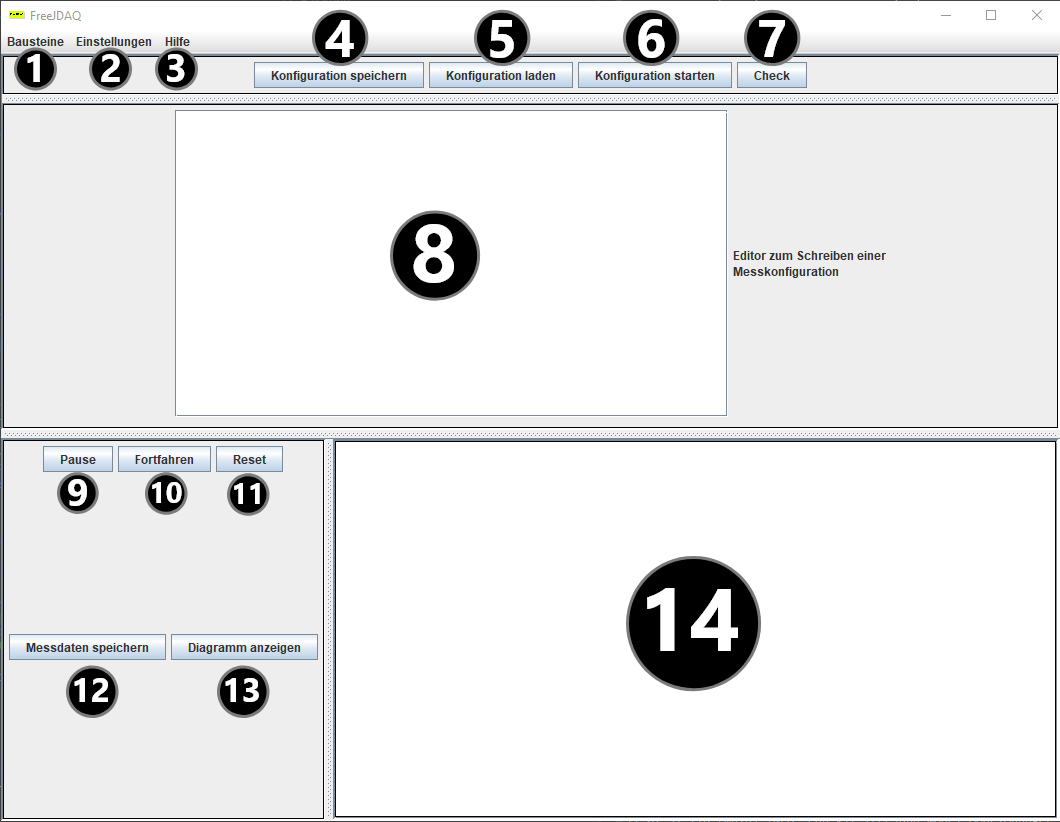
\includegraphics[width = 10cm]{Grafiken/Uebersicht_GUI_Mit_Nummern.png}
        \caption{Die Übersicht über die grafische Benutzeroberfläche von FreeJDAQ. Die Nummern verweißen auf die genauen Beschreibungen, die weiter unten zu finden sind.}
        \label{Uebersicht_GUI_Mit_Nummern}
    \end{center}
\end{figure}

\begin{enumerate}
    \item Bausteine
    
    \item Einstellungen
\end{enumerate}

\begin{flushleft}
    
\includegraphics[width = 2cm]{Grafiken/1-Bausteine.png}
\end{flushleft}

\begin{flushleft}
    
\includegraphics[width = 2cm]{Grafiken/2-Einstellungen.png}
\end{flushleft}

\begin{flushleft}
    
\includegraphics[width = 2cm]{Grafiken/3-Hilfe.png}
\end{flushleft}

\begin{flushleft}
    
\includegraphics[width = 2cm]{Grafiken/4-Konfiguration_speichern.png}
\end{flushleft}

\begin{flushleft}
    
\includegraphics[width = 2cm]{Grafiken/5-Konfiguration_laden.png}
\end{flushleft}

\begin{flushleft}
    
\includegraphics[width = 2cm]{Grafiken/6-Konfiguration_starten.png}
\end{flushleft}

\begin{flushleft}
    
\includegraphics[width = 2cm]{Grafiken/7-Check.png}
\end{flushleft}

\begin{flushleft}
    
\includegraphics[width = 2cm]{Grafiken/8-Editor.png}
\end{flushleft}

\begin{flushleft}
    
\includegraphics[width = 2cm]{Grafiken/9-Pause.png}
\end{flushleft}

\begin{flushleft}
    
\includegraphics[width = 2cm]{Grafiken/10-Fortfahren.png}
\end{flushleft}

\begin{flushleft}
    
\includegraphics[width = 2cm]{Grafiken/11-Reset.png}
\end{flushleft}

\begin{flushleft}
    
\includegraphics[width = 2cm]{Grafiken/12-Messdaten_speichern.png}
\end{flushleft}

\begin{flushleft}
    
\includegraphics[width = 2cm]{Grafiken/13-Diagramm_anzeigen.png}
\end{flushleft}

\begin{flushleft}
    
\includegraphics[width = 2cm]{Grafiken/14-Datenanzeige.png}
\end{flushleft}

\section{Beschreibung der Messkonfigurationssprache}

\section{Umgang mit dem Raspberry Pi}

\section{Fehlermeldungen}

\section{Limitierung der Anwendung}


\printnoidxglossaries				% generate pdf twice when adding new entries

\end{document}\grid
